\subsection{Security of Suffix Proofs} \label{proof_under_hard_fork}
In this section we revise the security proof for the Superblock NIPoPoWs suffix proof protocol provided in~\cite{nipopows}. In particular we revise Lemma~\ref{lemma:honest_vs_pure_adversarial_subchain} which lies in the heart of the security proof, as well as the security proof itself (Theorem~\ref{thm:suffix_security_soft_fork}). We also repeat any additional
definition and lemma needed for the security proof, aiming to provide extended and intuitive explanation for each one of them. Finally, we formally calculate an lower bound for the security parameter $m$ as a function of $k$.

Assume $t$ adversarial out of $n$ total parties, each with $q$ PoW random oracle
queries per round. We define $p = \frac{T}{2^\kappa}$ the probability of a
successful Random Oracle query. We will call a query to the RO $\mu$\textit{-successful}
if the RO returns a value $h$ such that $h \leq 2^{-\mu}T$.

We define the boolean random variables $X_r^{\mu}$, $Y_r^{\mu}$, $Z_r^{\mu}$.
Fix some round $r$, query index $j$ and adversarial party index $k$ (out of $t$).
If at round $r$ an honest party obtains a PoW with $id < 2^{-\mu}T$, set $X_r^{\mu} = 1$,
otherwise $X_r^{\mu} = 0$. If at round $r$ exactly one honest party obtains
$id < 2^{-\mu}T$, set $Y_r^{\mu} = 1$, otherwise $Y_r^{\mu} = 0$. If at round $
r$ the $j$-th query of the $k$-th corrupted party is $\mu$-successful, set
$Z_{rjk}^{\mu} = 1$, otherwise $Z_{rjk}^{\mu} = 0$. Let $Z_r^{\mu} =
\sum_{k=1}^t\sum_{j=1}^qZ_{rjk}^{\mu}$. For a set of rounds $S$, let
$X^\mu(S) = \sum_{r \in S}X^{\mu}_r$ and similarly define $Y_S^{\mu}$, $Z_S^{\mu}$.\\

\begin{defn}[Typical Execution]
	An execution of the protocol is $(\epsilon, \eta)$-typical if:
	
	\textbf{Block counts don't deviate.} For all $\mu \geq 0$ and any set
	$S$ of consecutive rounds with $\vert S \vert \geq 2^\mu \eta k$, we have:
	\begin{itemize}
		\item[-] $(1-\epsilon)E[X^\mu(S)] < X^\mu(S) < (1+\epsilon)E[X^\mu(S)] $ and
			$(1-\epsilon)E[Y^\mu(S)] < Y^\mu(S)$
		\item[-] $Z^\mu(S) < (1+\epsilon)E[Z^\mu(S)]$
\end{itemize}

	\textbf{Round count doesn't deviate.} Let $S$ be a set of consecutive rounds
	such that $X^\mu(S) \geq k$ for some security parameter $k$. Then $\vert S \vert
	\geq (1-\epsilon)2^\mu \frac{k}{pq(n-t)}$ with overwhelming probability.
	
	\textbf{Chain regularity.} No insertions, no copies and no predictions
	\cite{backbone} have occurred.
	\label{defn:typical_execution}
\end{defn}

\begin{thm}[Typicality]\label{thm:superblock_typicality}
	Executions are $(\epsilon, \eta)$-typical with overwhelming probability in $k$.
\end{thm}
\begin{proof}
	\textbf{Block counts and regularity.} We refer to \cite{backbone} for
	the full proof.

	\textbf{Round count.} First, observe that for a specific round $r$ we have $X_{r}
	\sim Bern(p)$, so for the $\mu$-level superblocks $X_{r}^\mu \sim Bern(2^{-\mu}p)$
	and these are independent trials. Therefore, since for $\vert S \vert$ rounds we
	have $(n-t)q\vert S \vert$ RO queries, we have that $X_S^\mu \sim
	\text{Bin}((n-t)q \vert S \vert, 2^{-\mu}p)$. So $(n-t)q \vert S \vert \sim
	\text{NB}(X_S^\mu, 2^{-\mu}p)$. Negative Binomial distribution is defined
	as $\text{NB}(r, p')$ and expresses the expected number of trials in a sequence of
	independent and identically distributed Bernoulli trials before a specified
	$(r)$ number of successes occurs. The expected total number of trials of a
	negative binomial distribution with parameters $(r, p')$ is $r/p'$. To see
	this, imagine an experiment simulating the negative binomial performed many
	times, that is a set of trials is performed until $r$ successes occur. Consider
	you perform $n$ experiments of total $N$ trials altogether. Now we would expect $Np' = nr$,
	so $N/n = r/p'$. See that $N/n$ is just the average number of trials per
	experiment. So we have $\mathbb{E}[(n-t)q \vert S \vert] = \frac{X^\mu_S}{2^{-\mu}p}
	\Rightarrow \mathbb{E}[\vert S \vert] = 2^\mu \frac{X^\mu_S}{(n-t)qp}$. If $X^\mu(S) \geq k$
	then we have that $\mathbb{E}[\vert S \vert] \geq 2^\mu \frac{k}{(n-t)qp}$ and we can apply a tail bound to the
	negative binomial distribution, so we obtain that $\text{Pr}[\vert S \vert < (1 -
	\epsilon)\mathbb{E}(\vert S \vert)] \in \Omega(\epsilon^{2}m)$.
\end{proof}

The following lemma lies in the heart of the formal security proof (Theorem~\ref{thm:suffix_security_soft_fork}). The revision of this lemma is one of our major contributions in this context, as it leads to revisions in the security proof theorem as well.

\begin{lemma}
	Suppose S is a set of consecutive rounds $r_1 \cdots r_2$
	and $\chain_B$ is a chain adopted by an honest party at round $r_2$ of a typical
	execution. Let $\chain^{B}_{S} = \{$ b $\in \chain_B:$ b was generated during $S\}$. Let
	$\mu_\mathcal{A}, \mu_B \in \mathbb{N}$. Suppose $\chain^{B}_{S}\upchain^{\mu_B}$ is good and suppose that $\vert \chain^S_B \upchain^{\mu_B} \vert \geq k$.
	Suppose $\chain_A$ is a $\mu_\mathcal{A}$-superchain containing only adversarial
	blocks generated during S. Then
	$2^{\mu_\mathcal{A}} \vert \chain_\mathcal{A} \vert <  2^{\mu_B} \vert    \chain^{B}_{S}\upchain^{\mu_B}\vert $.
	\label{lemma:honest_vs_pure_adversarial_subchain}
\end{lemma}
\begin{proof}
	From $\vert \chain^S_B \upchain^{\mu_B} \vert \geq k$ we have that $\vert X^{\mu_B}_S \vert \geq k$. 
	Applying Theorem~\ref{thm:superblock_typicality}, we conclude that  
	\begin{equation}\label{eq:honest_vs_pure_adversarial_subchain_eq1}
		\vert S \vert \geq (1-\epsilon)2^{\mu_B} \frac{\vert \chain^S_B \upchain^{\mu_B} \vert}{pq(n-t)}.
	\end{equation}
	%Applying the Chain Growth theorem~\cite{backbone} we obtain $\vert \chain_{B}^S \vert \geq (1 - \epsilon)f \vert S \vert$. 
	We also know from the goodness of $\chain_{B}^S \upchain^{\mu_B}$
	that 
	\begin{equation}\label{eq:honest_vs_pure_adversarial_subchain_eq2}
		\vert \chain_{B}^S \upchain^{\mu_B} \vert \geq (1 - \delta)2^{-\mu_B} \vert	\chain_{B}^S \vert
	\end{equation}
	So we have 
	\begin{equation}\label{eq:honest_vs_pure_adversarial_subchain_eq3}
		\lvert S \rvert \geq (1- \epsilon)(1- \delta) \dfrac{\lvert \chain^S_B \rvert}{pq(n-t)}
	\end{equation}
	For the number of $\mu_\mathcal{A}$-blocks that the adversary generated during $S$ we know that $\lvert \chain_\mathcal{A} \rvert \leq (1+\epsilon)2^{-\mu_\mathcal{A}} Z(S)$. But we know that $Z(S) < \dfrac{t}{n-t} \cdot \dfrac{f}{1-f} \lvert S \rvert + \epsilon f \lvert S \rvert $ so we have that 
	\begin{equation}\label{eq:honest_vs_pure_adversarial_subchain_eq4}
		\lvert \chain_\mathcal{A} \rvert < (1+\epsilon)2^{\mu_\mathcal{A}}( \dfrac{t}{n-t} \cdot \dfrac{f}{1-f} + \epsilon f) \lvert S \rvert
	\end{equation}

	By substituting \ref{eq:honest_vs_pure_adversarial_subchain_eq3} in \ref{eq:honest_vs_pure_adversarial_subchain_eq4} we have that
	\begin{equation}\label{eq:honest_vs_pure_adversarial_subchain_eq5}
		\lvert \chain_\mathcal{A} \rvert < (1+\epsilon)^2(1-\delta)2^{-\mu_\mathcal{A}}( \dfrac{t}{n-t} \cdot \dfrac{f}{1-f} + \epsilon f) \dfrac{\lvert \chain^S_B \rvert}{pq(n-t)}
	\end{equation}
	But from \ref{eq:honest_vs_pure_adversarial_subchain_eq2} we also know that $ \lvert \chain_{B}^S \rvert \leq \dfrac{2^{\mu_B}\lvert \chain_{B}^S \upchain^{\mu_B} \rvert}{1- \delta}$ and by substituting to~\ref{eq:honest_vs_pure_adversarial_subchain_eq5} we have that 
	\begin{equation}
		2^{\mu_\mathcal{A}} \lvert \chain_\mathcal{A} \rvert \leq (1+\epsilon)^2 ( \dfrac{t}{n-t} \cdot \dfrac{f}{1-f} + \epsilon f) \dfrac{2^{\mu_B}\lvert \chain^S_B \upchain^{\mu_B} \rvert}{pq(n-t)}
	\end{equation}

	So we conclude to $2^{\mu_\mathcal{A}} \vert \chain_\mathcal{A} \vert
	<  2^{\mu_B} \vert    \chain^{B}_{S}\upchain^{\mu_B}\vert $ considering that $\dfrac{f/(1-f)}{pq(n-t)} < \dfrac{1}{(1-\delta)(1+\epsilon)^2}$ .
\end{proof}

\begin{defn}[Adequate level of honest proof]
	Let $\pi$ be an
	honestly generated proof constructed upon some adopted chain $C$ and let $b \in 
	\pi $. Then $\mu'$ is defined as $\mu' = \max \{ \mu: \vert \pi\{b:\}\uparrow^{\mu}
	\vert \geq \max( m+1, (1-\delta)2^{-\mu} \vert \pi\{b:\}\uparrow^{\mu}\downarrow \vert )\}$.
	We call $\mu'$ the adequate level of proof $\pi$ with respect to block $b$ with
	security parameters $\delta$ and m. Note that the adequate level of a proof is a
	function of both the proof $\pi$ and the chosen block $b$.
\end{defn}


\begin{lemma}
	Let $\pi$ be some honest proof generated with security
	parameters $\delta$, m. Let C be the underlying chain, $b \in C$ be any block
	and $\mu'$ be the adequate level of the proof with respect to b and the same
	security parameters.\\Then $C\{b:\}\uparrow^{\mu'} = \pi\{b:\}\uparrow^{\mu'}$.
	\label{lemm:complete_adequate}
\end{lemma}
\begin{proof}
	$ \pi\{b:\}\uparrow^{\mu'} \subseteq C\{b:\}\uparrow^{\mu'}$ is
	trivial. For the converse, we have that in the iteration of the \emph{Prove for
	loop}\cite{nipopows} with $\mu = \mu^*$, the block stored in variable $B$
	precedes $b$ in $C$.

	Note that the Prover's for loop iterates over all levels in the interlink structure,
	and places in the proof all of the blocks that are of the corresponding level and succeed $B$ in $C$.

	Suppose $\mu = \mu^*$ is the first \emph{for} iteration during which the property
	is violated. This cannot be the first iteration since $B = C[0]$ and Genesis
	precedes all blocks. By induction hypothesis we see that during the iteration
	$\mu = mu^* + 1$, $B$ preceded $b$. From the definition of $\mu'$ we know that
	$\mu'$ is the highest level for which $\vert \pi\{b:\}\uparrow^{\mu} \vert
	\geq \max( m, (1-\delta)2^{-\mu} \vert \pi\{b:\}\uparrow^{\mu}\downarrow \vert ) $.

	Hence, this property cannot hold for $\mu^* > \mu$ and therefore $\vert
	\pi\{b:\}\uparrow^{\mu} \vert < m$ or $\neg$local-good$_\delta(\pi\{b:
	\}\uparrow \mu^*[1:], C, \mu^*)$.

	In case local-good is violated, variable $B$ remains unmodified and the induction
	step holds. If local-good is not violated, then $ \vert \pi\{b:\} \uparrow^{\mu^*}[1:]
	\vert < m$ and so $\pi\uparrow^{\mu^*}[-m]$, which is the updated value of $B$ at the
	end of $\mu^*$ iteration, precedes $b$.
\end{proof}

The intuition behind the adequate level is the following. Adequate is the level $\mu'$ of a proof $\pi$ with respect to block $b$, if this level is of good chain quality and doesn't miss any $\mu'$-superblock coming after $b$. Because of the goodness-aware prover algorithm~\ref{alg:goodness_aware_suffix_prover_soft_fork} each proof $\pi$ has an adequate level for every block $b \in \pi$.
Note that the adequate level is used in Claim 1a of the Security Proof (Theorem~\ref{thm:suffix_security_soft_fork}).\\

\begin{lemma}
	Suppose the verifier evaluates $\pi_\mathcal{A} \geq \pi_B$ in a
	protocol interaction where $B$ is honest and assume during the comparison that the
	compared level of the honest party is $\mu_B$. Let $b = LCA(\pi_\mathcal{A}, \pi_B)$ and
	let ${\mu}'_B$ be the adequate level of $\pi_B$ with respect to $b$. Then ${\mu}'_B
	\geq \mu_B$.
	\label{lemm:greatest_adequate}
\end{lemma}
\begin{proof}
	Because $\mu_B$ is the compared level of the honest party, from
	the definition of the $\geq_m$ operator, we have $2^{\mu_B} \vert \pi\{b:\}\uparrow^{\mu_B}
	\vert > 2^{{\mu}'_B} \vert \pi\{b:\}\uparrow^{{\mu}'_B} \vert $. This is true,
	otherwise the Verifier would have chosen level $\mu'_B$ as level of comparison.
	The proof is by contradiction. Suppose $\mu'_B < \mu_B$.
	By definition, $\mu'_B$ is the maximum level such that $\vert \pi_B\{b:\}\uparrow^\mu
	[1:] \vert \geq max(m, (1-\delta)2^{-\mu}\vert \pi_B\{b:\}\uparrow^\mu [1:]\downarrow
	\vert)$, therefore $\mu_B$ does not satisfy this condition.
	But we know that $\vert \pi_B\{b:\}\uparrow^\mu [1:] \vert > m$ because
	$\mu_B$ was selected by the Verifier.
	Therefore $ 2^{\mu_B} \vert \pi\{b:\}\uparrow^{\mu_B} \vert < (1-\delta)\vert
	\chain\{b:\}\vert $. \\
	But also $\mu'_B$ satisfies goodness, so $ 2^{\mu'_B} \vert \pi\{b:\}\uparrow^{\mu'_B}
	\vert > (1-\delta)\vert \chain\{b:\}\vert $.\\ From the last two equations we obtain
	$ 2^{\mu_B} \vert \pi\{b:\}\uparrow^{\mu_B} \vert < 2^{\mu'_B} \vert
	\pi\{b:\}\uparrow^{\mu'_B} \vert$ which contradicts the initial equation.
\end{proof}

The intuition behind the above lemma is the following. The comparison level chosen by the verifier can be
no other than the adequate level in respect to block $LCA(\pi_A, \pi_B)$, since
any other choice would be a level of non-good quality, because of the definition of
the adequate level. 
%%%%%   !!!!!!!     %%%%%%
% If you think about the adequate lemma could NEVER be higher than the chosen level of comparison 
So, in fact, a more accurate lemma should claim that $\mu'_B = \mu_B$. 
%%%%%%%%%%%%%%%%%%%%%%%%%%
Note that this lemma is used in the final step of Claim 3 in the security proof (Theorem~\ref{thm:suffix_security_soft_fork}).

\begin{thm}[Security of suffix proofs]
	Assuming honest majority, the non-interactive
	proofs-of-proof-of-work construction for computable $k$-stable monotonic
	suffix-sensitive predicates is secure with overwhelming probability in $k$.
	\label{thm:suffix_security_soft_fork}
\end{thm}
\begin{proof}
	By contradiction. Let $Q$ be a $k-$stable monotonic
	suffix-sensitive chain predicate. Assume NIPoPoWs on $Q$ is insecure. Then,
	during an execution at some round  $r_3$, $Q(\chain)$ is defined and the verifier
	$V$ disagrees with some honest participant. Assume the execution is typical.
	$V$ communicates with adversary $A$ and honest prover $B$. The verifier receives
	proofs $\pi_\mathcal{A}, \pi_B$. Because $B$ is honest, $\pi_B$ is a proof constructed
	based on underlying blockchain $\chain_B$ (with $\pi_B \subseteq \chain_B$), which $B$
	has adopted during round $r_3$ at which $\pi_B$ was generated. Furthermore,
	$\pi_\mathcal{A}$ was generated at round $r'_3 \leq r_3$.

	The verifier outputs $\neg Q(\chain_B)$. Thus it is necessary that $\pi_\mathcal{A} \geq 
	\pi_B$. We will show that this is a negligible event.

	Let $b_0 = LCA(\pi_\mathcal{A}, \pi_B)$. 
	Let $b^\star$ be the most recently honestly generated block in $\chain_B$ preceding $b$. Note that $b^\star$ necessarily exists because $\mathsf{Genesis}$ is honestly generated. 
	Let the levels of comparison
	decided by the verifier be $\mu_\mathcal{A}$ and $\mu_B$ respectively. Let $\mu'_B$
	be the adequate level of proof $\pi_B$  with respect to block $b_0$. Call
	$\alpha_\mathcal{A} = \pi_\mathcal{A} \uparrow^{\mu_\mathcal{A}}\{b_0:\}$,
	$\alpha'_B = \pi_B \uparrow^{\mu'_B}\{b_0:\}$.

	%%ANDRI:
	Note that the  proof parts succeeding block $b_0$ are the decisive ones 
	for the verifier's final choice. This is to adversary's advantage, since the parts 
	preceding this block demonstrate the proof-of-work contained in the common 
	(sub)chain, thus the adversary could only include equal or less PoW
	in her proof for this part of the chain.


	Our proof construction is based on the following intuition: we consider that $\alpha_\mathcal{A}$ consists of three distinct parts $\alpha_\mathcal{A}^1, \alpha_\mathcal{A}^2, \alpha_\mathcal{A}^3$ with the following properties.
	Block $b_0 = LCA(\pi_\mathcal{A}, \pi_B)$ is the fork point between $\pi_\mathcal{A} \upchain^{\mu_\mathcal{A}}, \pi_B \upchain^{\mu_B}$, as already defined.
	Let block $b_1 = LCA (\alpha_\mathcal{A}, \alpha'_B \downchain)$ be the fork point between $\alpha_\mathcal{A}$ and $\chain_B $ as an honest prover could observe. Then part $\alpha_\mathcal{A}^1$ contains the blocks between $b_0$ exclusive and $b_1$ inclusive, generated during the set of consecutive rounds $\mathcal{S}_1$ and also $\lvert  \alpha_\mathcal{A}^1 \rvert = k_1$.
	Consider $b_2$ the last block in $\alpha_\mathcal{A}$ that was generated by an honest party. Part $\alpha_{\mathcal{A}}^2$ contains the blocks between $b_1$ exclusive and $b_2$ inclusive generated during the set of consecutive rounds $\mathcal{S}_2$ and $\vert  \alpha_\mathcal{A}^2 \vert = k_2$.
	Consider $b_3$ the next block of $b_2$ in $\alpha_\mathcal{A}$. Then $\alpha_{\mathcal{A}}^3 = \alpha_\mathcal{A}[b_3{:}]$ and $\vert  \alpha_\mathcal{A}^3 \vert = k_3$ consisting of adversarial blocks generated during the set of consecutive rounds $\mathcal{S}_3$. Therefore $\vert \alpha_\mathcal{A} \vert = k_1 + k_2 + k_3$ and we will show that $\vert \alpha_\mathcal{A} \vert < \vert \alpha_B \vert$.

	We will now show three successive claims: First, $\alpha^1_\mathcal{A}$ and $\alpha'_B \downchain$ have only a few blocks in common. Second, $a^2_\mathcal{A}$ contains only a few blocks.
	And third, the adversary is able to produce this $a_\mathcal{A}$ with negligible probability.

	\noindent
	\textbf{Claim 1:} $\alpha_\mathcal{A}, \alpha'_B\downchain$ have only a few blocks in common. 

	\noindent
	We show this by taking the two possible cases for the relation of $\mu_\mathcal{A}$, $\mu'_B$.

	\noindent
	\textit{\underline{Claim 1a}:} If $\mu'_B \leq \mu_\mathcal{A}$ then they are completely
	disjoint. In such a case of inequality, every block in $\alpha_\mathcal{A}$ would also be
	of lower level $\mu'_B$. Applying Lemma~\ref{lemm:complete_adequate} to $C\{b:\}\upchain^{\mu'_B}$  we see
	that $\chain\{b:\}\upchain^{\mu'_B} = \pi\{b:\}\upchain^{\mu'_B}$. Subsequently, any
	block in $\pi_\mathcal{A}\upchain^{\mu_\mathcal{A}}\{b:\}[1:]$ would also be included in proof
	$\alpha'_B$, but $b=LCA(\pi_\mathcal{A}, \pi_B)$ so there can be no succeeding block
	common in $\alpha_\mathcal{A}, \alpha'_B$.
	
	\noindent
	\textit{\underline{Claim 1b}:} If  $\mu'_B > \mu_\mathcal{A}$ then $\vert \alpha_\mathcal{A}[1:] 
	\cap \alpha'_B\downarrow[1:] \vert = k_1$ where $k_1 \leq 2^{\mu'_B - \mu_\mathcal{A}}$.\\
	Let's call $b'$ the first block in $\alpha'_B$ after block $b_0$.
	Suppose for contradiction that $k_1 > 2^{\mu'_B - \mu_\mathcal{A}}$.  Since $\chain_B^{\mu'_B}$ is
	of good chain quality, this would mean that block $b'$, of level $\mu'_B$ is also
	of level $\mu_\mathcal{A}$. Since it is of level $\mu_\mathcal{A}$ the adversary could include it in
	the proof but $b'$ cannot exist in both $\alpha_\mathcal{A}, \alpha'_B$ since $\alpha_\mathcal{A}
	\cap \alpha'_B = \emptyset$ by definition. In case that the adversary chooses not
	to include $b'$ in the proof then she can include no other blocks of $\chain_B$ in
	her proof, since it would not consist a valid chain. Thus wehave reached to a contradiciton in either way.

	From Claim $1a$ and Claim $1b$, we conclude that there are $\vert \alpha_\mathcal{A}
	\vert - k_1$ blocks after block $b_0$ in $\alpha_\mathcal{A}$ which do not exist in $\alpha_B\downchain$.\\

	The intuition behind Claim 1b is that the common blocks of $\alpha^1_\mathcal{A}, \alpha'_B\downchain$ may only be blocks of level $\mu_\mathcal{A}$ which precede the first $\mu'_B$ block appearing in $\alpha'_B$. If $b'$ is included in the adversary's proof, then $b'$ would be the LCA of $\alpha_\mathcal{A}, \alpha'_B$, which violates the minimality of $b_0$. If it is not, then the adversary could include no more blocks from the common part of chain $\chain_B$ in her proof, since they would no longer form a valid interlinked chain in $\alpha_\mathcal{A}$. The quantity $2^{\mu'_B - \mu_\mathcal{A}}$ should be thought as follows: in the range between two consequent $\mu'_B$-level blocks, we have $n = 2^{\mu'_B}$ 0-level blocks and, thus, $2^{-\mu_\mathcal{A}}n = 2^{\mu'_B - \mu_\mathcal{A}}$ blocks of $\mu_\mathcal{A}$-level. 
	
	Before stepping into Claim 2 remember that we have defined block $b_1 = LCA(\alpha'_B \downchain, \alpha_\mathcal{A})$. This makes $b_1$
	the last block before the 0-level fork point, included in the adversary's proof.

	\noindent
	\textbf{Claim 2:} $a^2_\mathcal{A}$ contains only a few blocks.

	\noindent
	We show this by showing that $\alpha_\mathcal{A}[k_1 + k_2 + 1:]$ contains no honestly generated
	blocks due to the Common Prefix property. Suppose for contradiction that the block $\alpha_\mathcal{A}[i]$ for some $i \geq k_1 +
	k_2 + 1$ was honestly generated. This means that an honest party adopted the chain
	$\alpha_\mathcal{A}[:i - 1]\downarrow$ at some round $r_2 \leq r_3$. Because of the way honest
	parties adopt chains, the superchain $\alpha_\mathcal{A}[:i - 1]$ has an underlying properly
	constructed 0-level anchored chain $\chain_\mathcal{A}$ such that $\alpha_\mathcal{A}[:i - 1] \subseteq \chain_\mathcal{A}$.
	Let $j$ be the index of block $b_1$ within $\alpha_\mathcal{A}$, $j_\downarrow$ be the index
	of block $b_2$ within $\chain_\mathcal{A}$ and $k_{2\downarrow} = \vert \alpha_\mathcal{A}[j:j+k_2]\downarrow\vert$.
	See Figure \ref{fig:proof} for a demonstration. Observe that $\vert \chain_\mathcal{A}[:\{\alpha_\mathcal{A}[i-1]\}]
	\vert \geq \vert \chain_\mathcal{A}[:{j_\downarrow}+k_{2\downarrow}] \vert$, while
	$\chain_\mathcal{A}[j_\downarrow:j_\downarrow + k_{2\downarrow}] \npreceq \chain_B$ as proved in
	Claim 1. But $\chain_\mathcal{A}$ was adopted by an honest party at round $r_2$, which is prior
	to round $r_3$ during which $\chain_B$ was adopted by an honest party B. This 
	contradicts the Common Prefix\cite{backbone} with parameter $k_{2\downarrow}$. It follows that with overwhelming probability in $k_{2\downarrow}$, the 
	$k_3 = \vert \alpha_\mathcal{A} \vert - k_2 - k_1$ last blocks of the adversarial proof have been adversarially generated.\\

	\begin{figure}[h]
		\begin{center}
			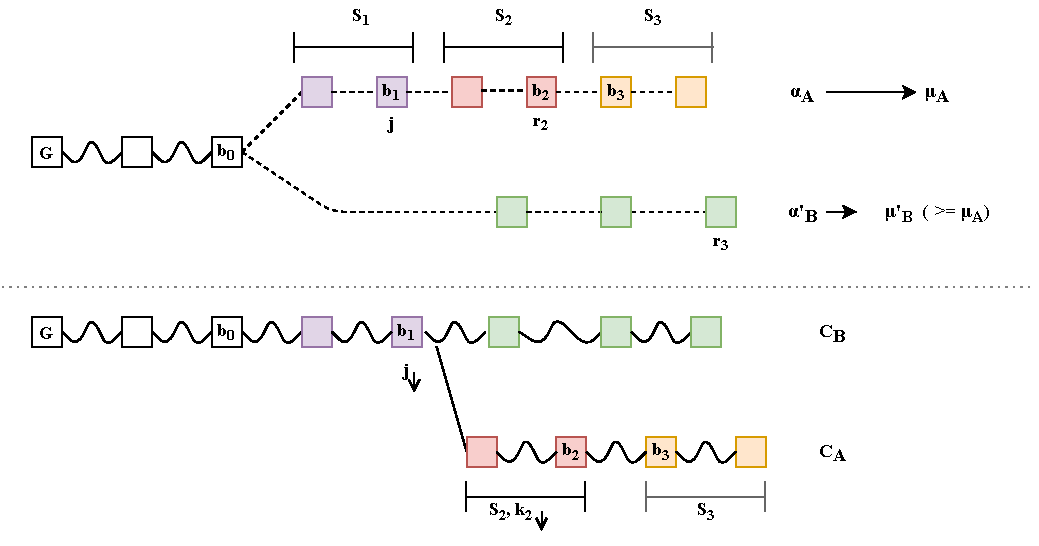
\includegraphics[width=\columnwidth]{figures/proof.pdf}
		\end{center}
		\caption{Two competing proofs at different levels. At the bottom the
		corresponding 0-level chains are represented.}
		\label{fig:proof}
	\end{figure}

	The intuition behond Claim 2 is that because of Common Prefix on $k_{2\downarrow}$ parameter, where
	$k_{2\downarrow} = \vert \alpha_\mathcal{A}[j:j+k_2]\downarrow\vert$, and because
	$\mathbb{E}[k_{2\downarrow}] = 2^{\mu_\mathcal{A}}k_2$, there can be no honest party adopting
	$\chain_\mathcal{A}$ at any round $i \geq k_1 + k_2 + 1$. \\

Before stepping into Claim 3 remember that we have defined block $b_2$ the last honestly generated block in $\alpha_\mathcal{A}$. $b_2$ is equal to $b^\star$ if no such block exists in $\alpha_\mathcal{A}$. Remember also that $b_3$ is the next block of $b_2$ in $\alpha_\mathcal{A}$, as shown in Figure~\ref{fig:proof}.

	\noindent
	\textbf{Claim 3:} Adversary $\mathcal{A}$ is able to produce $\alpha_\mathcal{A}$ that wins against $\alpha_B$ with negligible probability.

	\noindent
	Let $r_1$ the round when $b_3$ was generated.
	Consider the set $S_3$ of consecutive rounds $r_1..r_3$. Every block in
	$\alpha_\mathcal{A}[-k_3:]$ has been adversarially generated during $S_3$ and $\vert
	\alpha_\mathcal{A}[-k_3:] \vert = \vert \alpha_\mathcal{A}\{b_3:\} \vert = k_3$. $\chain_B$ is a chain
	adopted by an honest party at round $r_3$ and filtering the blocks by the rounds
	during which they were generated to obtain $\chain_B^S$, we see that if $b'$ is the
	most recently generated block in $\alpha_B$ in a round $r \leq r_1$, then $\chain_B^S =
	\chain_B\{ b': \}$. But $\chain_B^S \uparrow^{\mu'_B}$ is good with respect to $\chain_B^S$.
	Applying Lemma 1, we obtain that with overwhelming probability  $2^{\mu_\mathcal{A}} \vert
	\alpha_\mathcal{A}\{b_3:\} \vert < 2^{\mu'_B} \vert \chain_B^S \uparrow^{\mu'_B} \vert$, which is
	equal to

	\begin{equation}
	2^{\mu_\mathcal{A}} \vert \alpha_\mathcal{A}\{b_3:\} \vert < 2^{\mu'_B} \vert \alpha'_B\{b':\} \vert
	\end{equation} 

	since $\alpha'_B$ contains all the $\mu'_B$-level blocks in $\chain_B^S$. \\

	In order to complete the proof, let us now consider $\alpha_\mathcal{A}^{k_1}$,
	$\alpha_\mathcal{A}^{k_2}$, $\alpha_\mathcal{A}^{k_3}$ the parts of $\alpha_\mathcal{A}$ where the
	$k_1$, $k_2$, $k_3$ blocks reside and $\alpha_B^{k_1}$, $\alpha_B^{k_2}$,
	$\alpha_B^{k_3}$ the parts of $\alpha_B$ containing blocks generated in the
	corresponding round sets as illustrated in Figure \ref{fig:claim3}.

	\begin{figure}[h]
		\begin{center}
			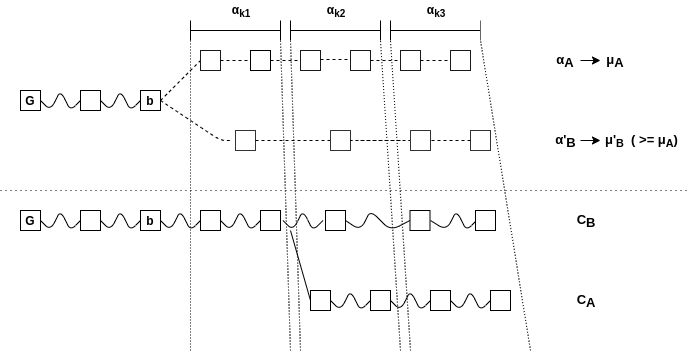
\includegraphics[width=0.9\columnwidth]{figures/claim3.png}
		\end{center}
		\caption{The three round sets in two competing proofs at different levels.
		The vertical dashed lines denote the area of interest, across proofs and chains,
		corresponding to each round set. At the bottom the corresponding 0-level chains
		are represented.}
		\label{fig:claim3}
	\end{figure}

	Subsequently to the above Claims we have that:

	Because of the common underlying chain in the first round set $S_1$:
	\begin{equation} \label{eq_round_set_1}
	2^{\mu_\mathcal{A}} \vert \alpha^1_\mathcal{A} \vert \leq 2^{\mu'_B} \vert \alpha'^1{_B} \vert
	\end{equation}

	Because of the adoption by an honest party of chain $\chain_B$ at a later round $r_3$, 
	we have for the second round set $S_2$:
	\begin{equation} \label{eq_round_set_2}
	2^{\mu_\mathcal{A}} \vert \alpha^2_\mathcal{A} \vert \leq 2^{\mu'_B} \vert \alpha'^2{_B} \vert
	\end{equation}

	Because of Equation (1), we have for the third round set:
	\begin{equation} \label{eq_round_set_3}
	2^{\mu_\mathcal{A}} \vert \alpha^3_\mathcal{A} \vert < 2^{\mu'_B} \vert \alpha'^3{_B} \vert
	\end{equation}

	So we have

	\begin{equation*}
	2^{\mu_\mathcal{A}} ( \vert \alpha^1_\mathcal{A} \vert + \vert \alpha^2_\mathcal{A} \vert + \vert
	\alpha^3_\mathcal{A} \vert ) < 2^{\mu'_B} ( \vert \alpha'^1{_B} \vert + \vert
	\alpha'^2{_B} \vert + \vert \alpha'^3{_B} \vert)
	\end{equation*}

	and finally
	\begin{equation}
	2^{\mu_\mathcal{A}} \vert \alpha_\mathcal{A} \vert < 2^{\mu'_B} \vert \alpha'{_B} \vert
	\end{equation}


	Therefore we have proven that $2^{\mu'_B} \vert \pi_B \uparrow^{\mu'_B} \vert >
	2^{\mu_\mathcal{A}} \vert \pi_\mathcal{A}^{\mu_\mathcal{A}} \vert$. From the definition of $\mu_B$, we know
	that $2^{\mu_B} \vert \pi_B \uparrow^{\mu_B} \vert > 2^{\mu'_B} \vert \pi_B
	\uparrow^{\mu'_B} \vert$ because it was chosen $\mu_B$ as level of comparison
	by the Verifier. So we conclude that $2^{\mu_B} \vert \pi_B \uparrow^{\mu_B}
	\vert > 2^{\mu_\mathcal{A}} \vert \pi_\mathcal{A} \uparrow^{\mu_\mathcal{A}} \vert$.

\end{proof}

It remains to calculate the security parameter $m$ that guarantee that all the above
hold true in every implementation. It suffices to compute a security parameter
value for each set of rounds $k_1, k_2, k_3$, so that the proof equations
\ref{eq_round_set_1}, \ref{eq_round_set_2}, \ref{eq_round_set_3} hold and
then sum these values to obtain parameter $m$.

In the first set of rounds, for the first $k_1$ blocks in $\alpha_\mathcal{A}$, we only need
one block included in $\alpha_B$ for the part of the proof described in Equation
\ref{eq_round_set_1}. In the second set of rounds we need $2^{-\mu_B}\kappa$ blocks
for the part of the proof described in Equation \ref{eq_round_set_2}, just as it
directly results from the Common Prefix property. In order to make $m$ independent
of any specific level it suffices to consider the upper bound of $\kappa$ blocks
for this set of rounds. In the last set of rounds we need at least $\kappa$
adversarially generated blocks in $\alpha_\mathcal{A}^{k_3}$ so that Lemma 1 is applicable.
Since we assume honest majority, obliging to at least $\kappa$ blocks for this
set of rounds suffices to guarantee for Equation \ref{eq_round_set_3}.

So, we finally conclude to the following upper bound for the value of the
security parameter:
\begin{equation}
	m = 2k + 1
\end{equation}